\section{Experiments}
\label{sec:experiments}

\subsection{Datasets and baselines}
\label{sec:data}
To validate our method, we evaluate its performance on the publically available dataset used in~\cite{lejeune18}. This consists several video and volumes of different modalities with 2D annotation points for different object types. Briefly, it includes:
\begin{itemize}
\item[-]{\bf{Brain:}} $4$ 3D T2-weighted MRI scans from the publicly available BRATS challenge dataset~\cite{menze15}, where tumors are object of interest
\item[-]{\bf{Tweezer:}} $4$ sequences from the training set of the publicly dataset MICCAI Endoscopic Vision challenge: Robotic Instruments segmentation~\cite{endochal}. The piecewise-rigid surgical instrument must be segmented.
  
\item[-]{\bf{Slitlamp:}} $4$ slit-lamp video recordings of human retinas, where the optic disk is to be segmented. 

\item[-]{\bf{Cochlea:}} $4$ volumes of 3D CT scans of the inner ear, where the cochlea must be annotated. This object is the most challenging object to segment due to its complicated geometry. 
\end{itemize}

To this, we evaluate the following methods:
\begin{itemize}
\item[-]{\bf Gaze2Segment:} A combination of saliency detection and graphcut~\cite{khosravan16}. 
\item[-]{\bf DL-prior:} Point location supervision is used to train a CNN with strong object priors~\cite{bearman16}.
\item[-]{\bf EEL:} An expected exponential loss to learn robust classifiers in a PU learning setting~\cite{lejeune17}. 
\item[-]{\bf KSPTrack:} Multiple-instance tracking method described in~\cite{lejeune18}. 
\item[-]{\bf KSPTrack/GMM:} Our approach with entrance and transition costs computed according to Eq.~\eqref{eq:bc}.
\item[-]{\bf KSPTrack/DEC} Our approach using the proposed Deep Embedded Clustering described above.
\end{itemize}

\subsection{Experiments}
\subsubsection{Accuracy of segmentations}
Table \ref{tab:results} shows on each baseline the F1 score between the generated segmentation and the corresponding groundtruth annotation.
Figure \ref{fig:qualitative} shows for each sequence type graphical example.
Note that our clustering approach tends to improve the foreground probability maps (second vs. fifth column).

\begin{table}
\centering
\caption{
Quantitative results on all datasets. We report the F1 scores and standard deviations.
}
\label{tab:results}
\begin{tabular}{llp{1.8cm}p{1.8cm}p{1.8cm}p{1.8cm}p{1.8cm}}
\toprule
Types &                 Brain &               Cochlea &              Slitlamp &               Tweezer \\
Methods             &                       &                       &                       &                       \\
\midrule
KSPTrack/DEC/fg/var &       $0.76 \pm 0.08$ &       $0.55 \pm 0.04$ &       $0.62 \pm 0.08$ &       $0.76 \pm 0.09$ \\
KSPTrack/DEC/fg     &       $0.76 \pm 0.08$ &       $0.38 \pm 0.33$ &        $0.6 \pm 0.05$ &       $0.72 \pm 0.09$ \\
KSPTrack/DEC        &       $0.75 \pm 0.08$ &       $0.55 \pm 0.07$ &       $0.66 \pm 0.05$ &        $0.79 \pm 0.1$ \\
KSPTrack/GMM        &  $\bm{0.79} \pm 0.06$ &       $0.54 \pm 0.03$ &       $0.63 \pm 0.07$ &  $\bm{0.81} \pm 0.06$ \\
\hdashline
KSPTrack            &       $0.74 \pm 0.08$ &  $\bm{0.66} \pm 0.02$ &  $\bm{0.77} \pm 0.08$ &       $0.77 \pm 0.08$ \\
EEL                 &       $0.52 \pm 0.14$ &       $0.12 \pm 0.05$ &       $0.59 \pm 0.08$ &        $0.6 \pm 0.16$ \\
DL-prior            &       $0.56 \pm 0.08$ &        $0.3 \pm 0.04$ &       $0.51 \pm 0.11$ &       $0.72 \pm 0.06$ \\
Gaze2Segment        &       $0.07 \pm 0.02$ &       $0.07 \pm 0.02$ &        $0.02 \pm 0.0$ &        $0.18 \pm 0.0$ \\
\bottomrule
\end{tabular}
\end{table}


\begin{figure}[h!]
\centering
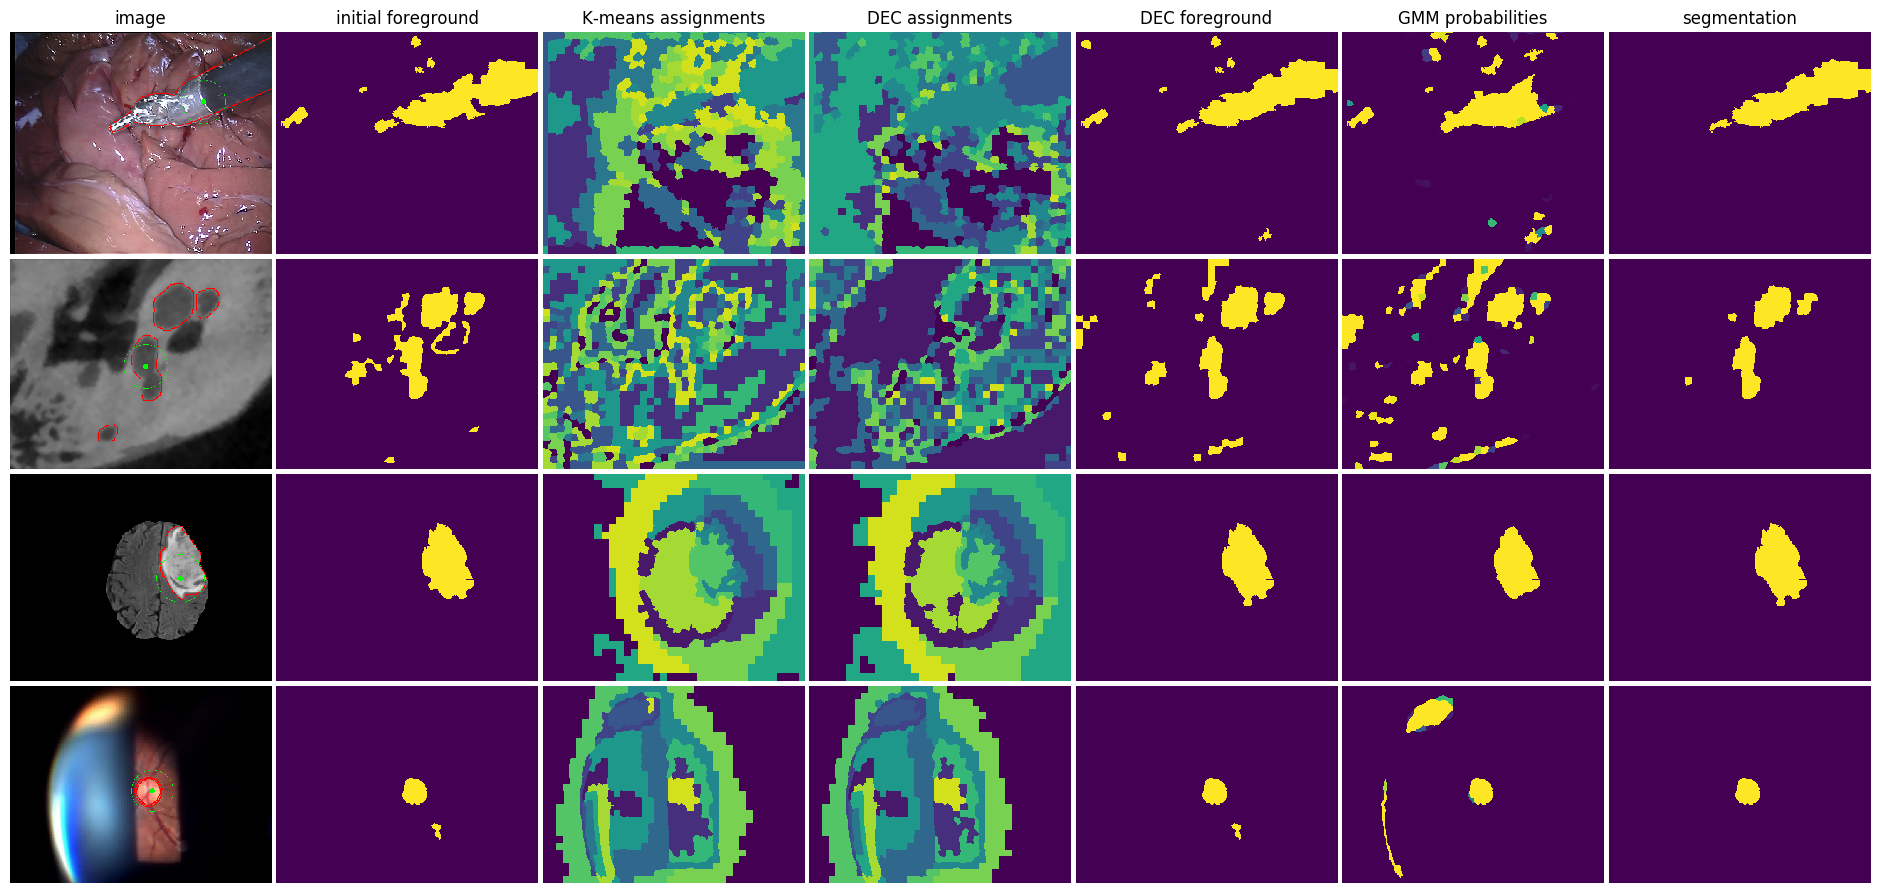
\includegraphics[width=1.\textwidth]{prevs}
\caption{Qualitative results showing from left to right: (1) Original frame with ground truth contour in red and 2D location in green. The entrance region is the outer circle (2) Thresholded foreground probabilities using plain autoencoder's features. (3) Clusters from K-means. (4) Clusters after DEC. (5) Thresholded foreground probabilities with optimal features. (6) Entrance probabilities given user input of column 1. (7) Final segmentation}
\label{fig:qualitative}
\end{figure}


%%% Local Variables:
%%% mode: latex
%%% TeX-master: "../../main"
%%% End:
